\section{Introduction}

This chapter presents the complete architectural design of VidChain and its intelligence engine, IRIS. Every structural decision documented here was made in response to one of the three core problems identified in Chapter 1: the Context Window Wall, Sensory Hallucination and Action Flickering, and the lack of Temporal Entity Persistence. The architecture is examined at four levels of abstraction: a high-level overview, a component breakdown, a class hierarchy, and a runtime sequence trace, each supported by a formal diagram.

\section{Architectural Philosophy: Late-Fusion}

The central architectural decision in VidChain is the adoption of a \textbf{Late-Fusion} paradigm for multimodal data processing. This is a deliberate departure from the Early-Fusion approach used by most state-of-the-art Video-Language Models \cite{videollava}, where raw visual tokens are concatenated with text tokens and fed jointly into a single large transformer.

Early-Fusion presents two fundamental problems on edge hardware. First, the combined token budget of vision and language far exceeds what a 4\,GB VRAM device can hold in a single forward pass. Second, it creates a single point of failure: if the visual encoder produces noisy output, a common occurrence on low-quality footage, that noise propagates directly into the language model's context and cannot be corrected.

Late-Fusion instead processes each modality through an independent, specialised expert node. Each node produces a structured text log, referred to as a Sensor Log, that is human-readable and verifiable. These logs are only merged at the RAG retrieval stage \cite{rag}, after each modality has been individually validated and filtered. A failure in the OCR node, for example, simply produces a null entry in the timeline rather than corrupting the vision or audio streams.

The practical consequence is that VidChain can run a Vision Language Model \cite{moondream}, a Whisper transcription engine \cite{whisper}, and an EasyOCR reader on the same 4\,GB GPU without any of them competing for the same memory window at the same time.

\section{Architecture Overview}

\subsection{Diagram}

\begin{figure}[H]
\centering
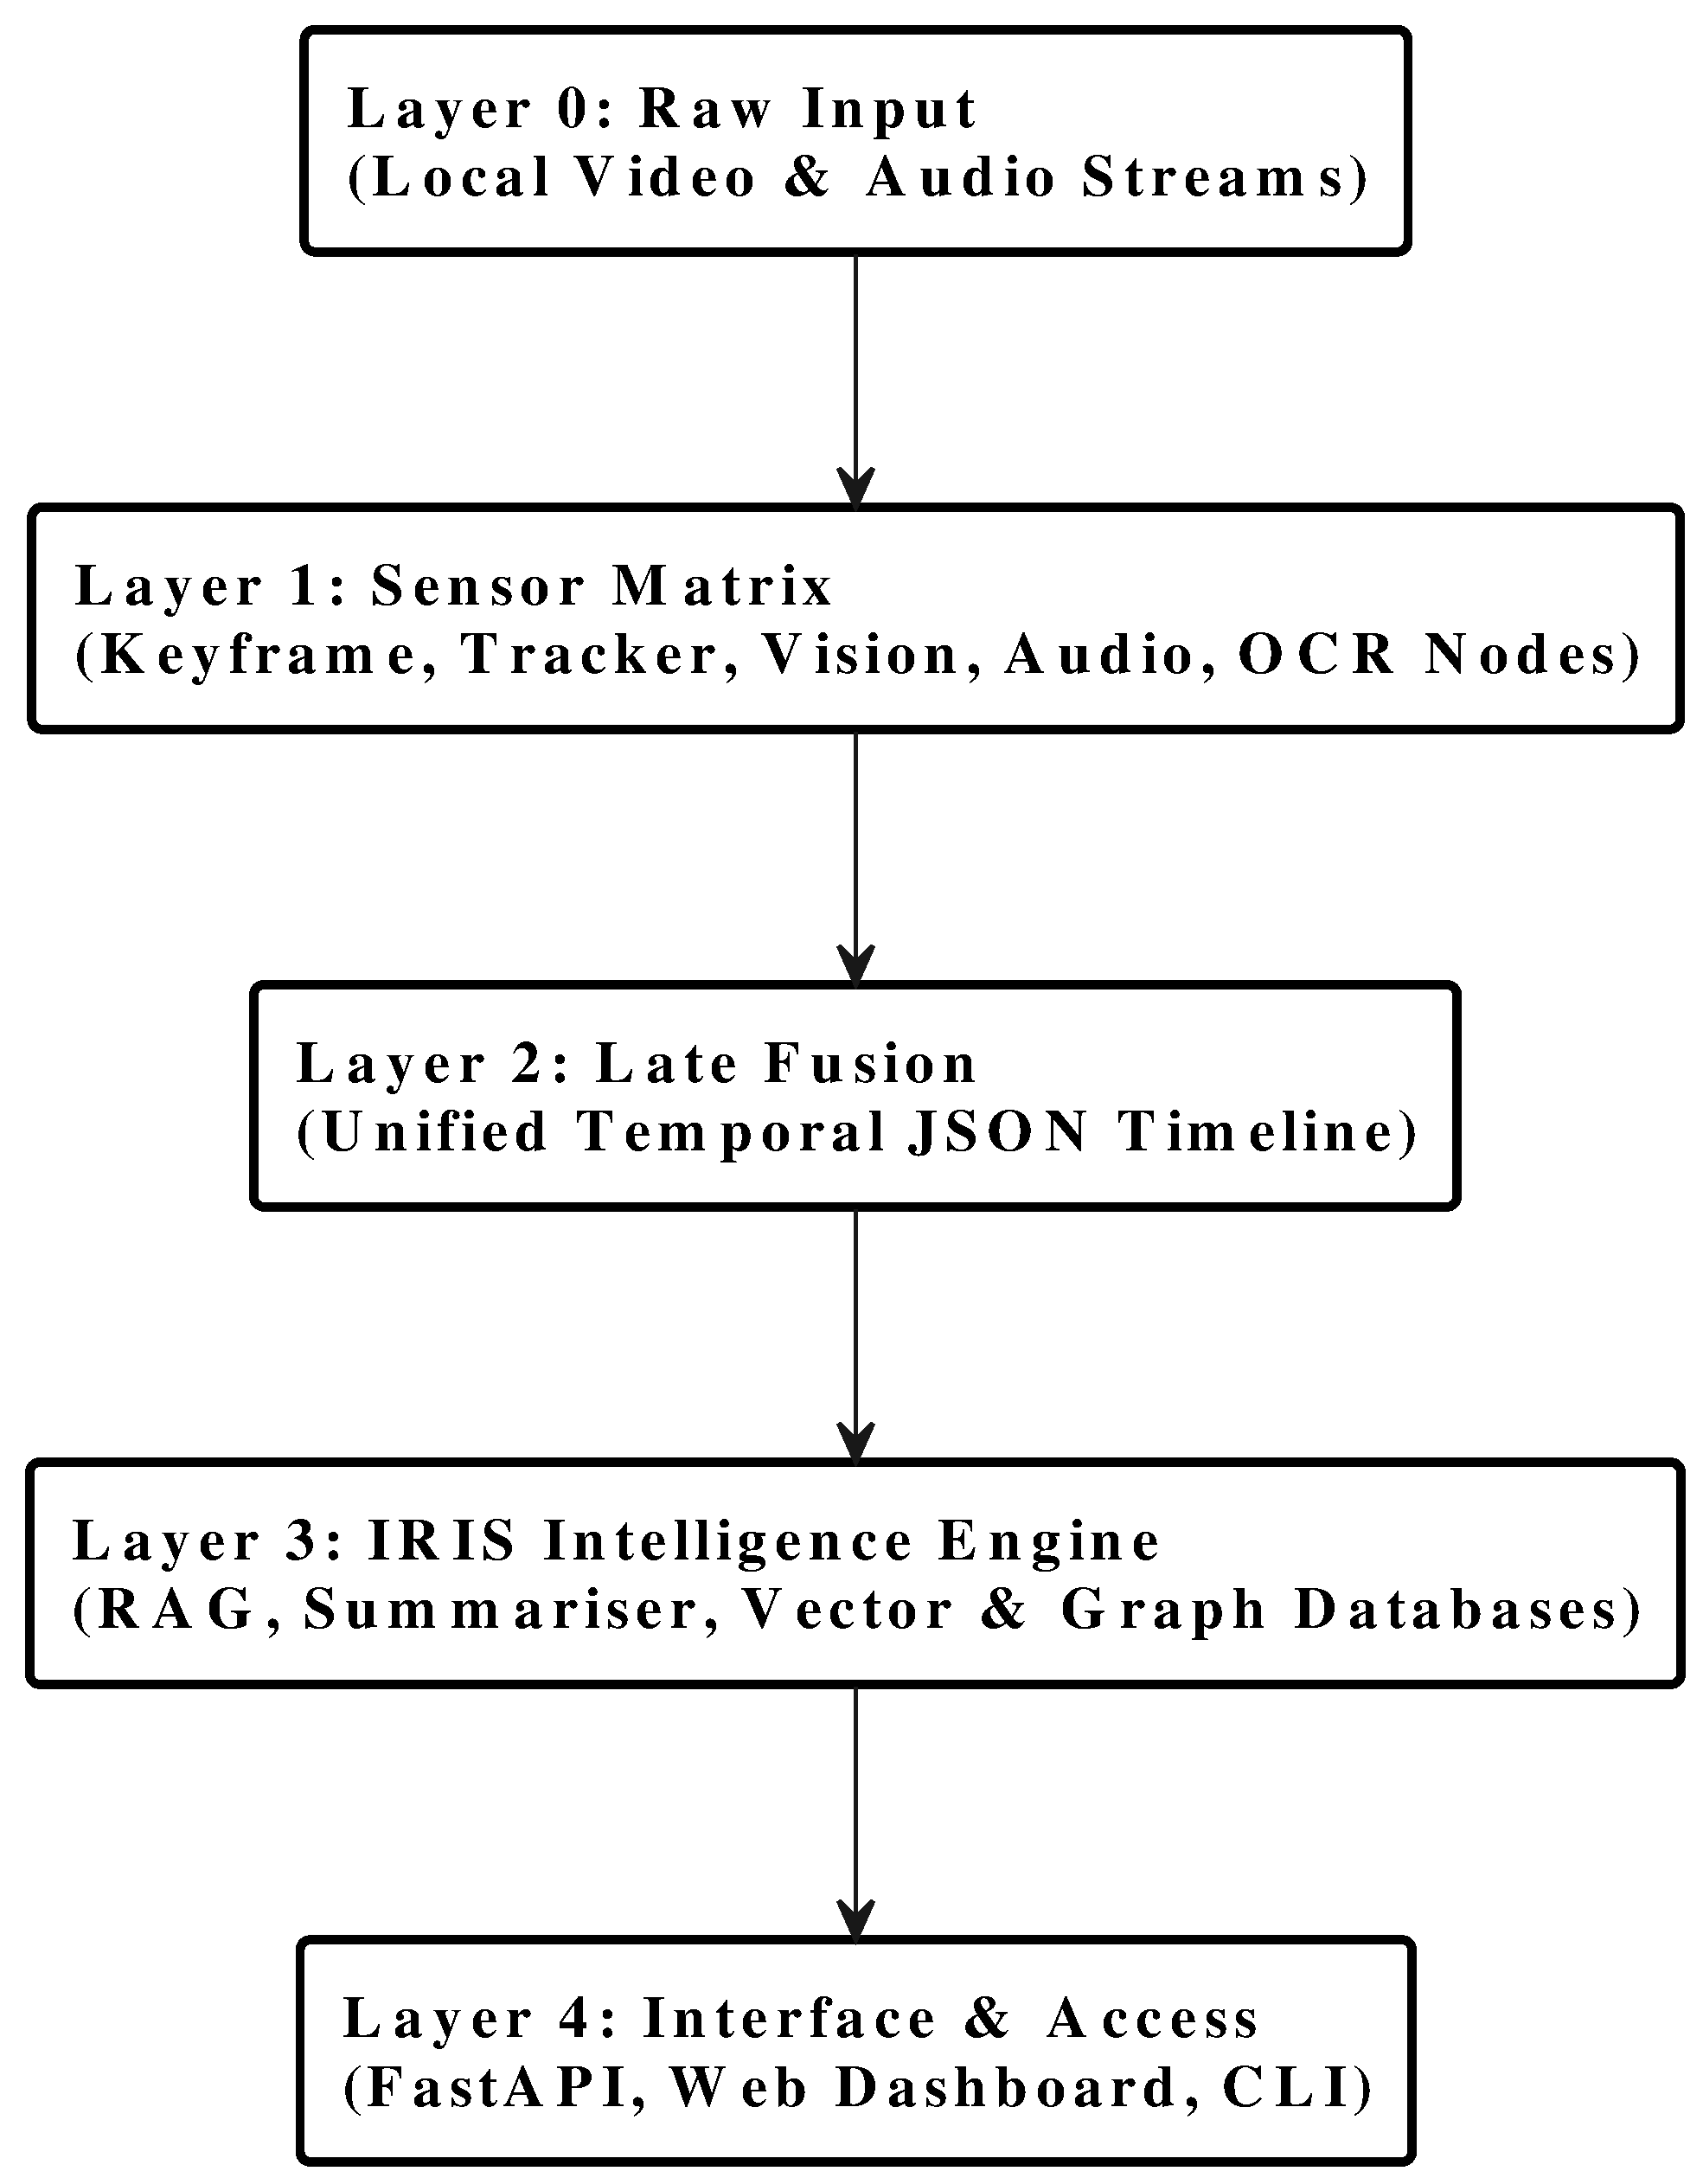
\includegraphics[width=0.85\textwidth]{architecture.pdf}
\caption{VidChain Four-Layer Architecture Overview}
\label{fig:arch_overview}
\end{figure}

\subsection{Layer Descriptions}

VidChain is organised into four vertical layers, each with a single, well-defined responsibility.

\textbf{Layer 0 (Raw Input)} accepts a local video file path. No preprocessing is required from the user. The \texttt{VideoChain} orchestrator handles audio extraction, frame decoding, and FPS normalisation internally.

\textbf{Layer 1 (Sensor Matrix)} is the core processing layer. It is composed of composable \texttt{BaseNode} implementations that each extract one modality from the video. Nodes are stateless with respect to each other and communicate only through a shared context dictionary, never through direct references. This means any node can be removed, replaced, or reordered without breaking the pipeline.

\textbf{Layer 2 (Late Fusion)} is not a separate module but a structural contract. After all nodes have processed a frame, the shared context dictionary is serialised into a unified timeline entry containing every modality's output for that timestamp in a single flat structure, which becomes the unit of storage for both ChromaDB \cite{chromadb} and the Knowledge Graph.

\textbf{Layer 3 (IRIS Intelligence Engine)} is responsible for all reasoning. It comprises four sub-components: the ChromaDB vector store for semantic similarity search, the Temporal Knowledge Graph for entity-level relational reasoning, the RAG Engine with cross-encoder reranking for query resolution, and the Map-Reduce Summariser \cite{mapreduce} for long-form narrative generation.

\textbf{Layer 4 (Interface)} exposes the system through four access points: a FastAPI edge server as the primary integration point, the IRIS Web Portal built in Next.js, the VidChain Studio desktop application, and the \texttt{vidchain-analyze} CLI for headless use.

\section{Data Flow Diagram}

The data flow is presented at two levels of abstraction. Figure~\ref{fig:dfd0} shows the Level-0 Context Diagram, illustrating the system boundaries and the interactions between the VidChain Intelligence System and external entities: the Researcher (providing queries and receiving insights), Local Storage (supplying raw media), and the AI Inference Models (performing neural processing).

\begin{figure}[H]
\centering
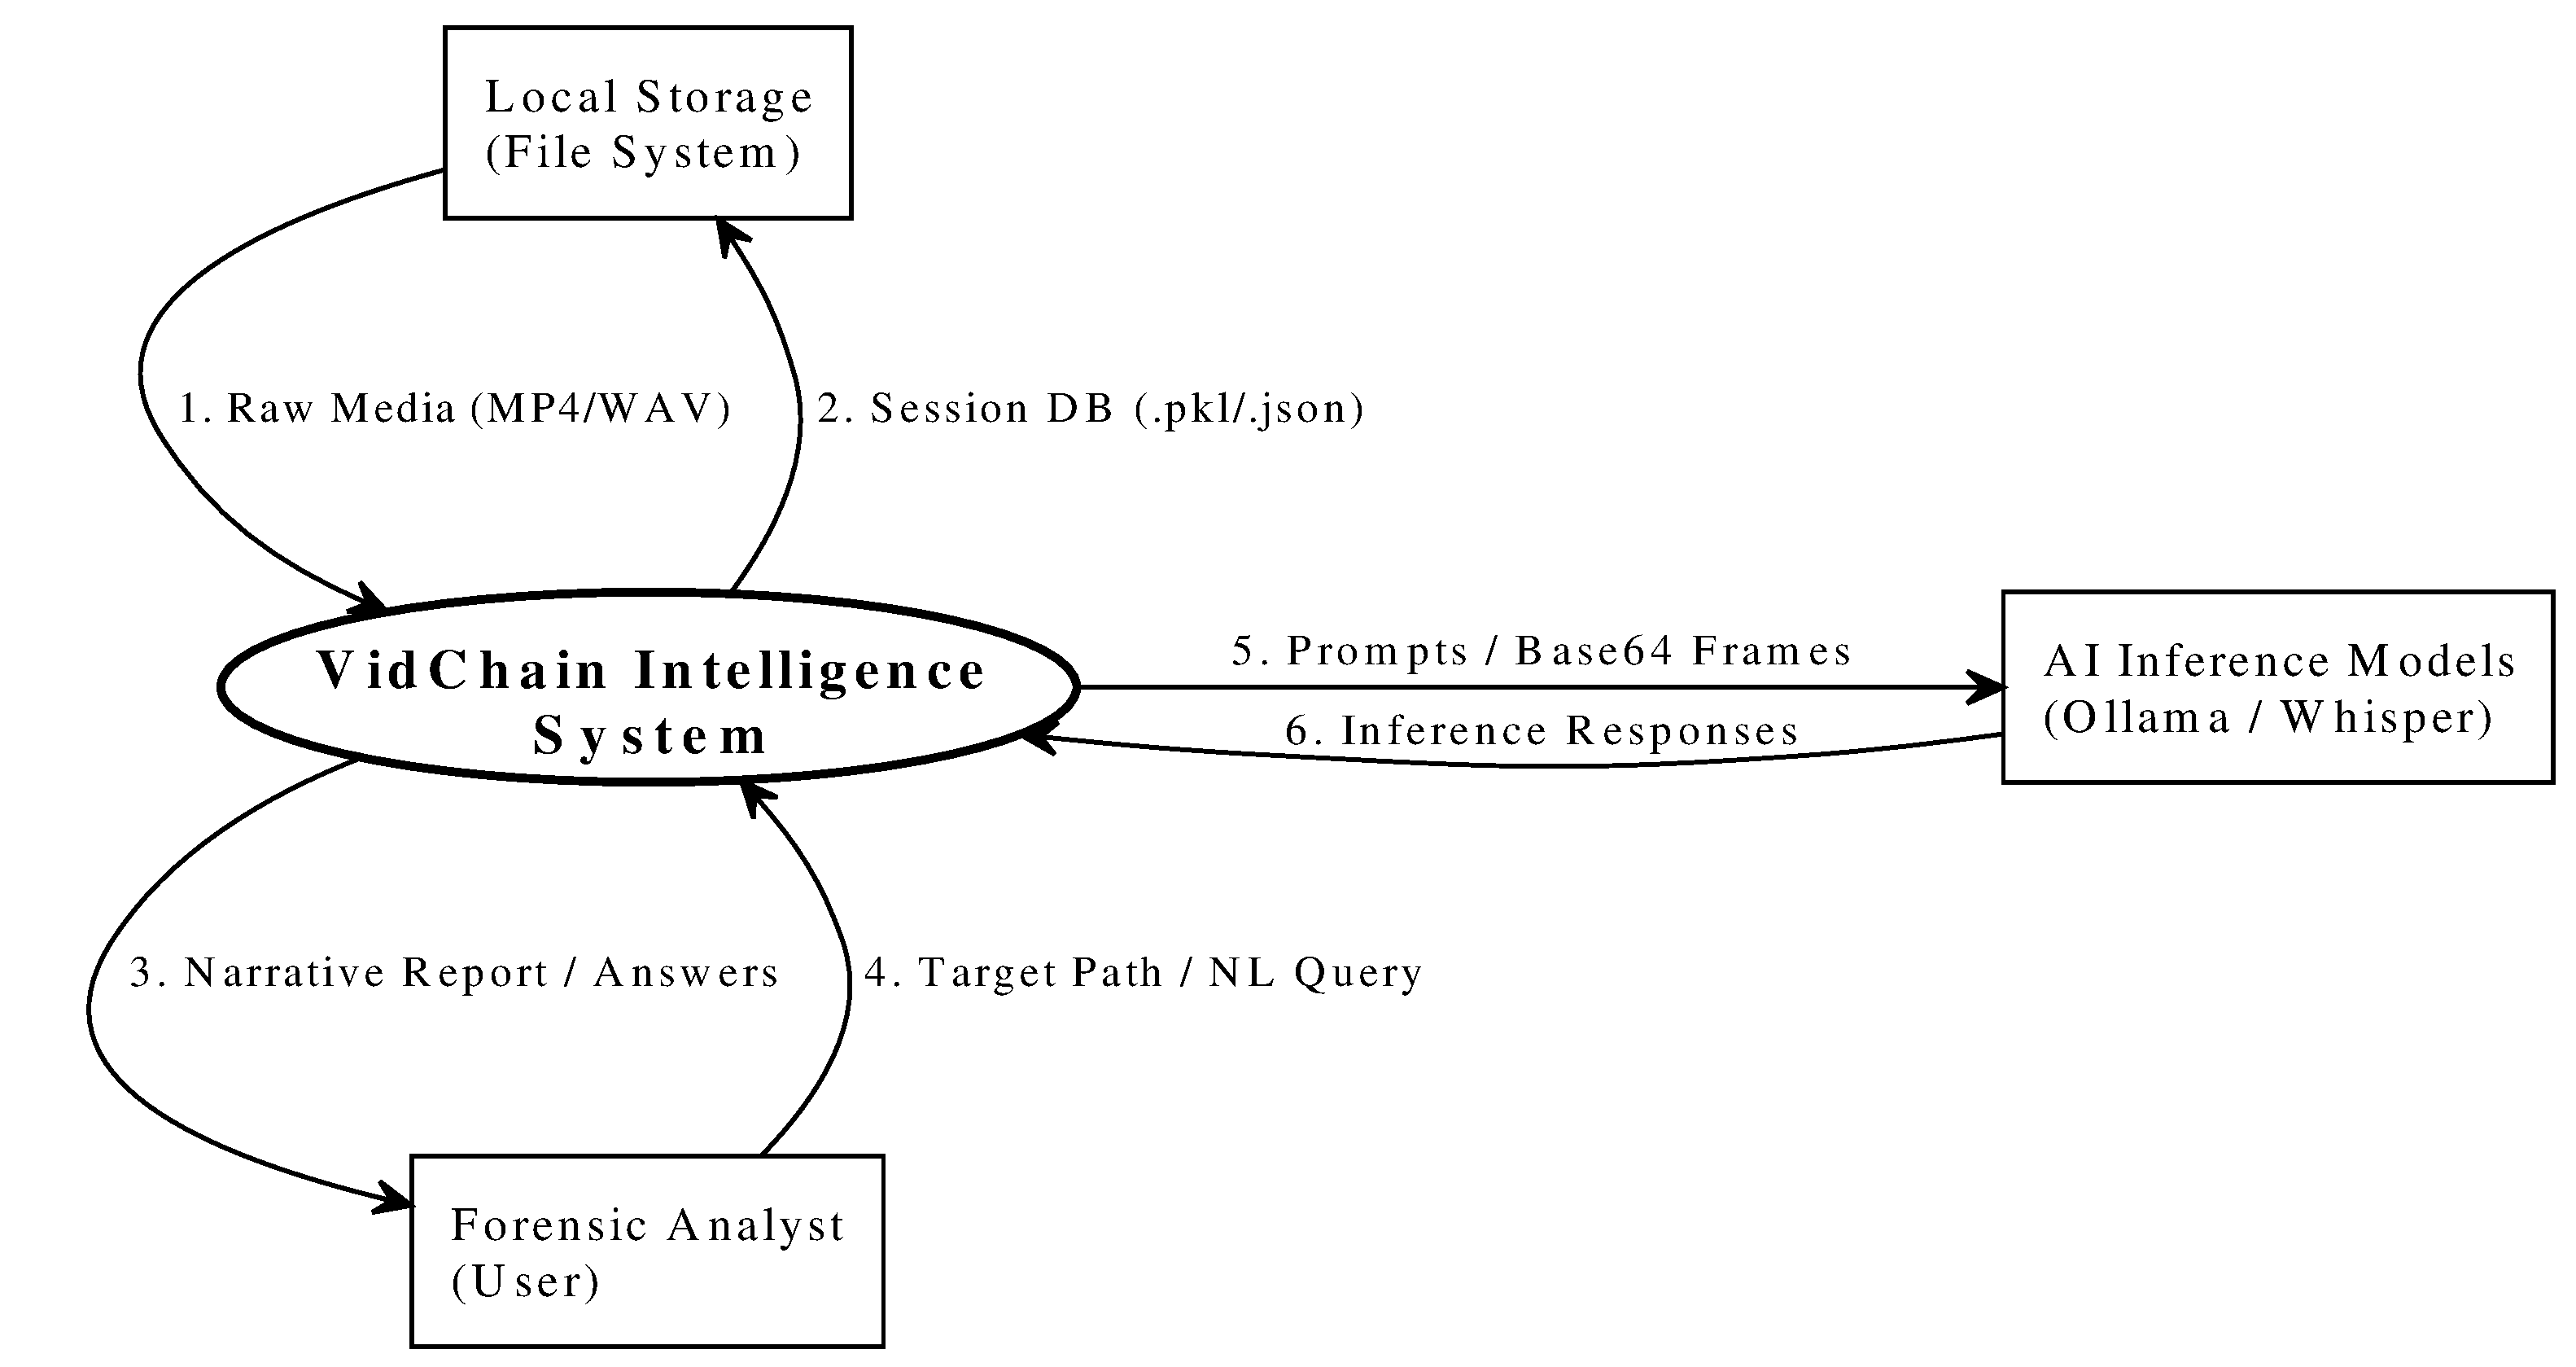
\includegraphics[width=\textwidth]{DFD-0.pdf}
\caption{Level-0 Context Diagram --- VidChain System Boundary}
\label{fig:dfd0}
\end{figure}

Figure~\ref{fig:dfd} shows a Level-1 DFD of the VidChain processing pipeline. A raw video file enters the \texttt{VideoChain} orchestrator (P1), which passes frames through the \texttt{AdaptiveKeyframeNode} (P2) and the \texttt{TrackerNode} (P3) before distributing keyframes to the four primary sensor nodes: \texttt{WhisperNode} (P4), \texttt{LlavaNode} (P5), \texttt{OcrNode} (P6), and the Action and Emotion nodes (P7, P8). Each node returns a structured Sensor Log to the orchestrator for Late Fusion. The fused timeline is indexed into ChromaDB (D1), the Local Knowledge Graph (D2), and the Global Knowledge Graph (D3). The RAG Engine (P9) reads from all three stores to resolve queries, and the Map-Reduce Summariser (P10) consumes context chunks from P9 to produce the final narrative report returned to the researcher.

\begin{figure}[H]
\centering
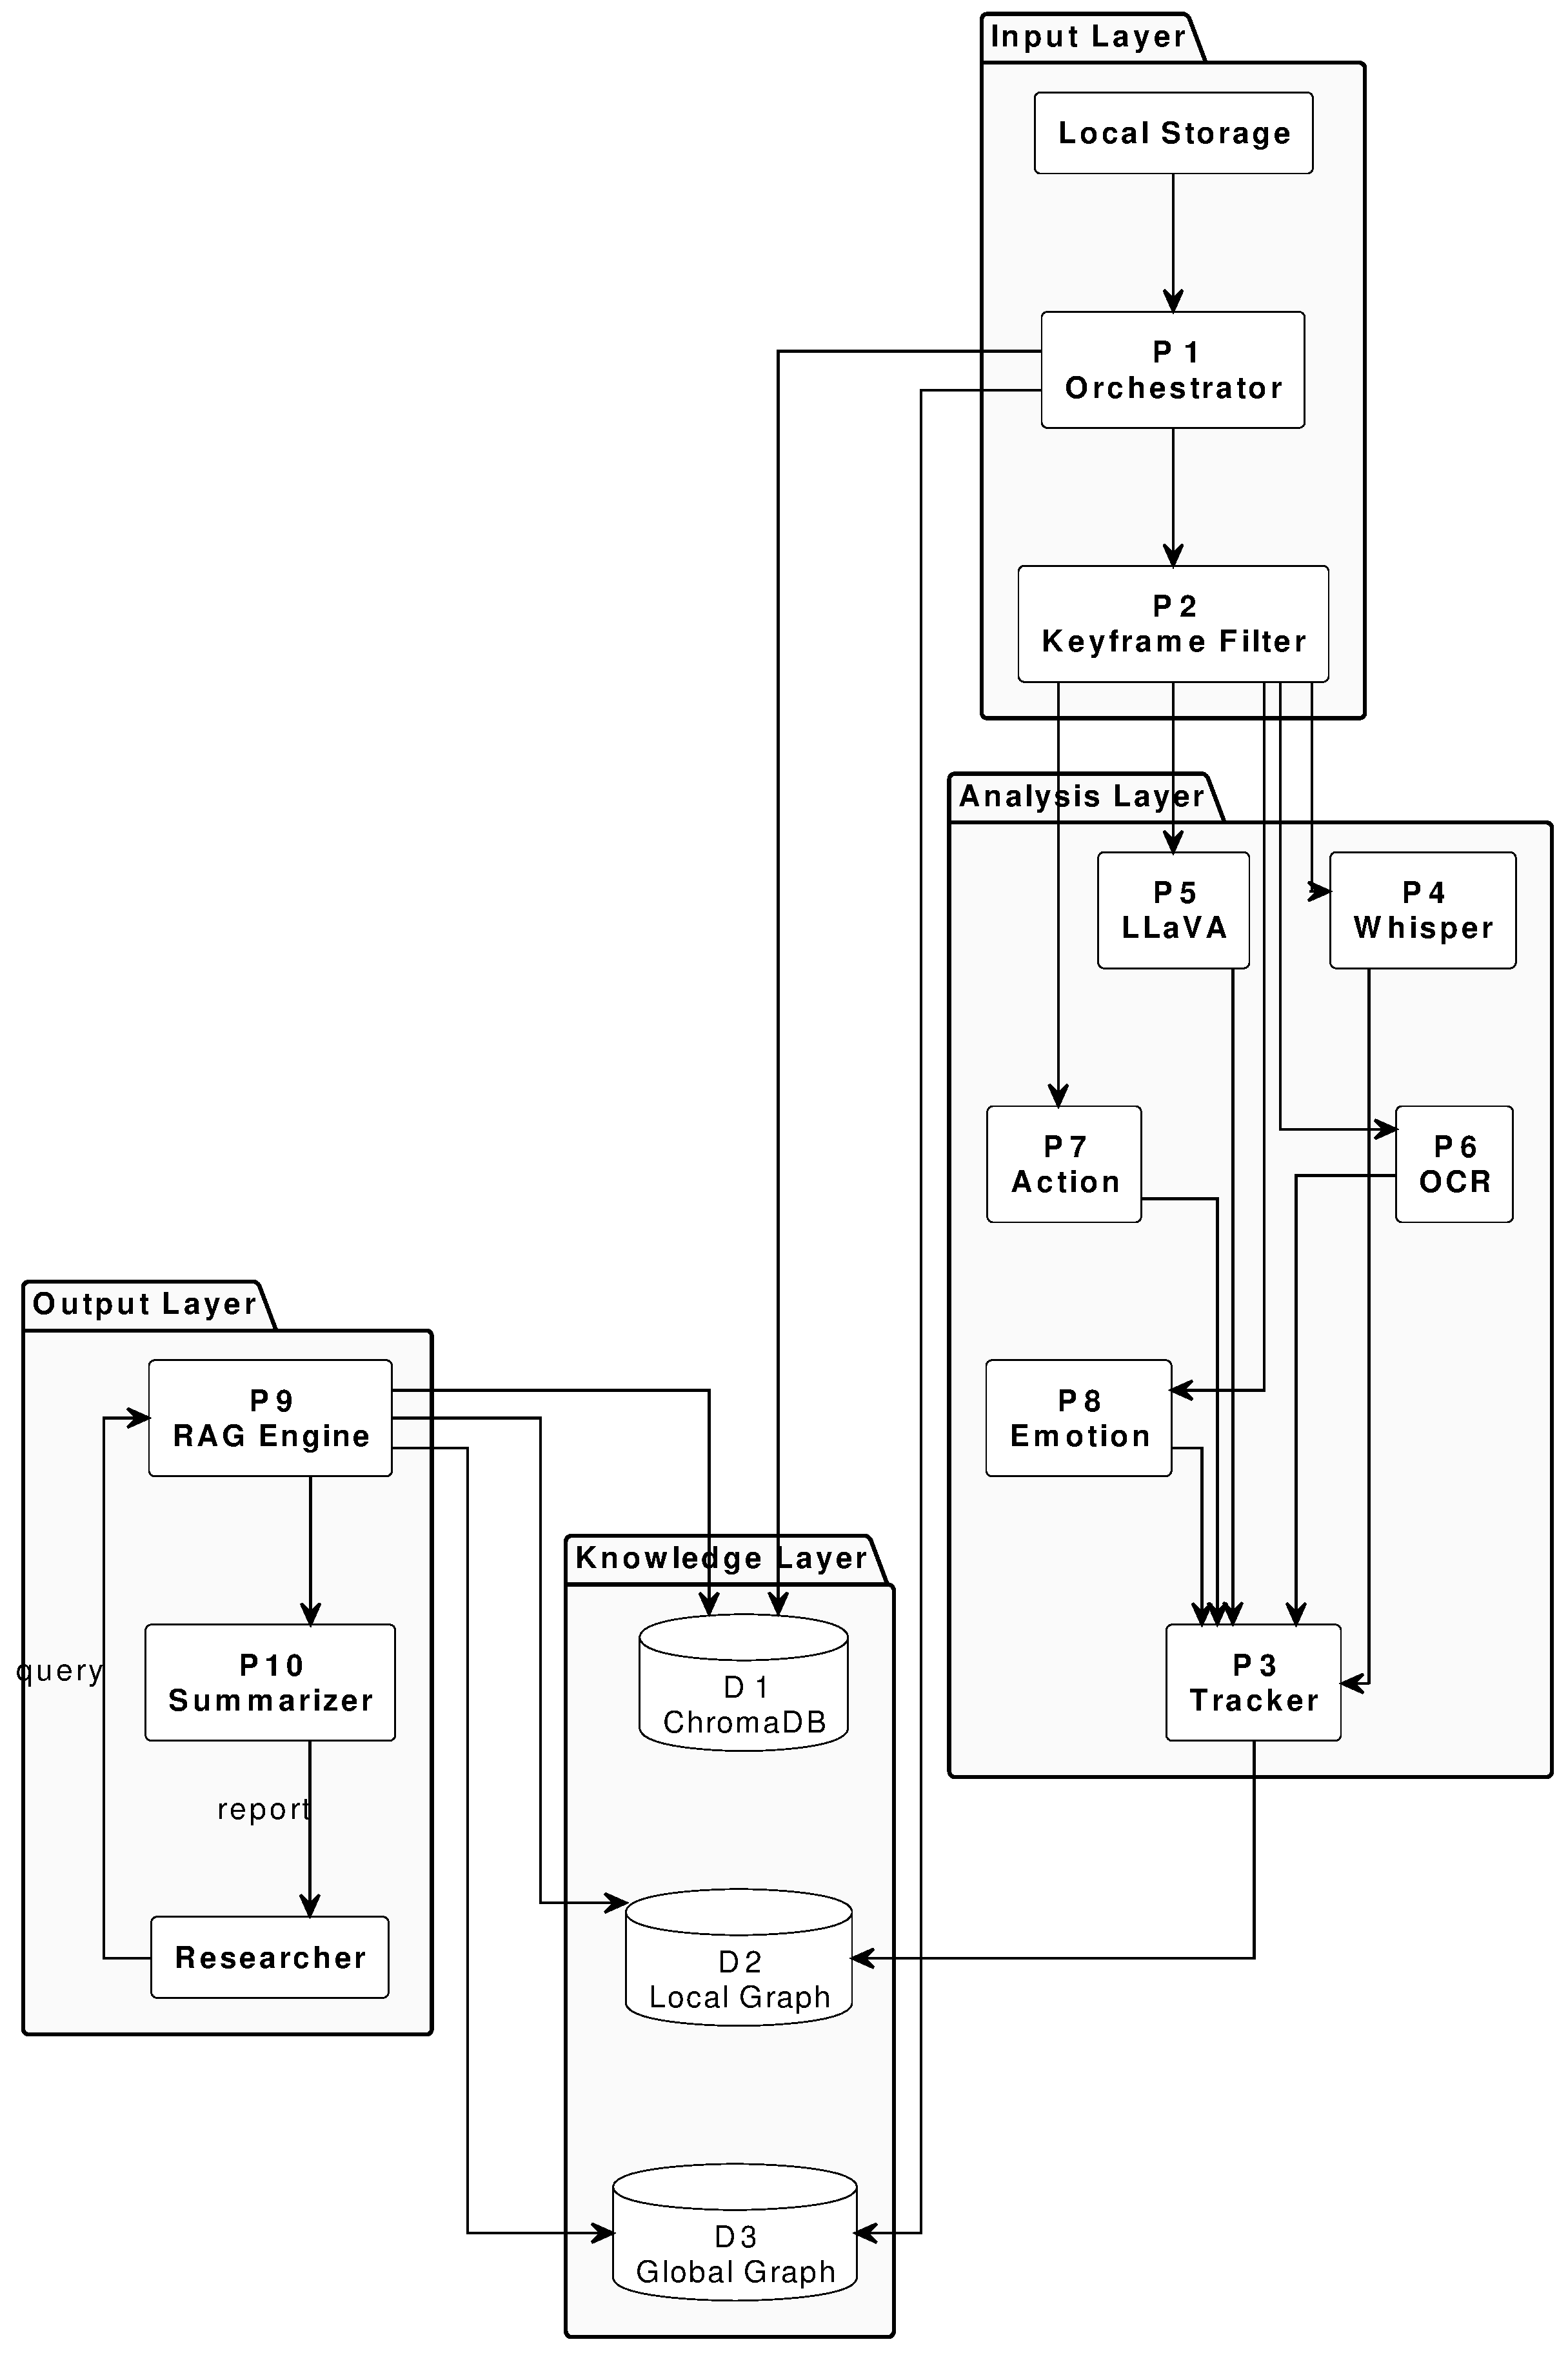
\includegraphics[width=\textwidth]{DFD-1.pdf}
\caption{Level-1 Data Flow Diagram --- VidChain Multimodal Processing Pipeline}
\label{fig:dfd}
\end{figure}

\section{Process Flow: Ingestion Pipeline}

Figure~\ref{fig:ingest_flow} traces the frame-by-frame execution path through the ingestion pipeline, from initial video capture through keyframe filtering, multimodal sensor processing, metadata fusion, and final storage into the vector and graph databases.

\newgeometry{left=0.2cm, right=0.2cm, top=0.2cm, bottom=0.2cm}
\begin{sidewaysfigure}
\centering
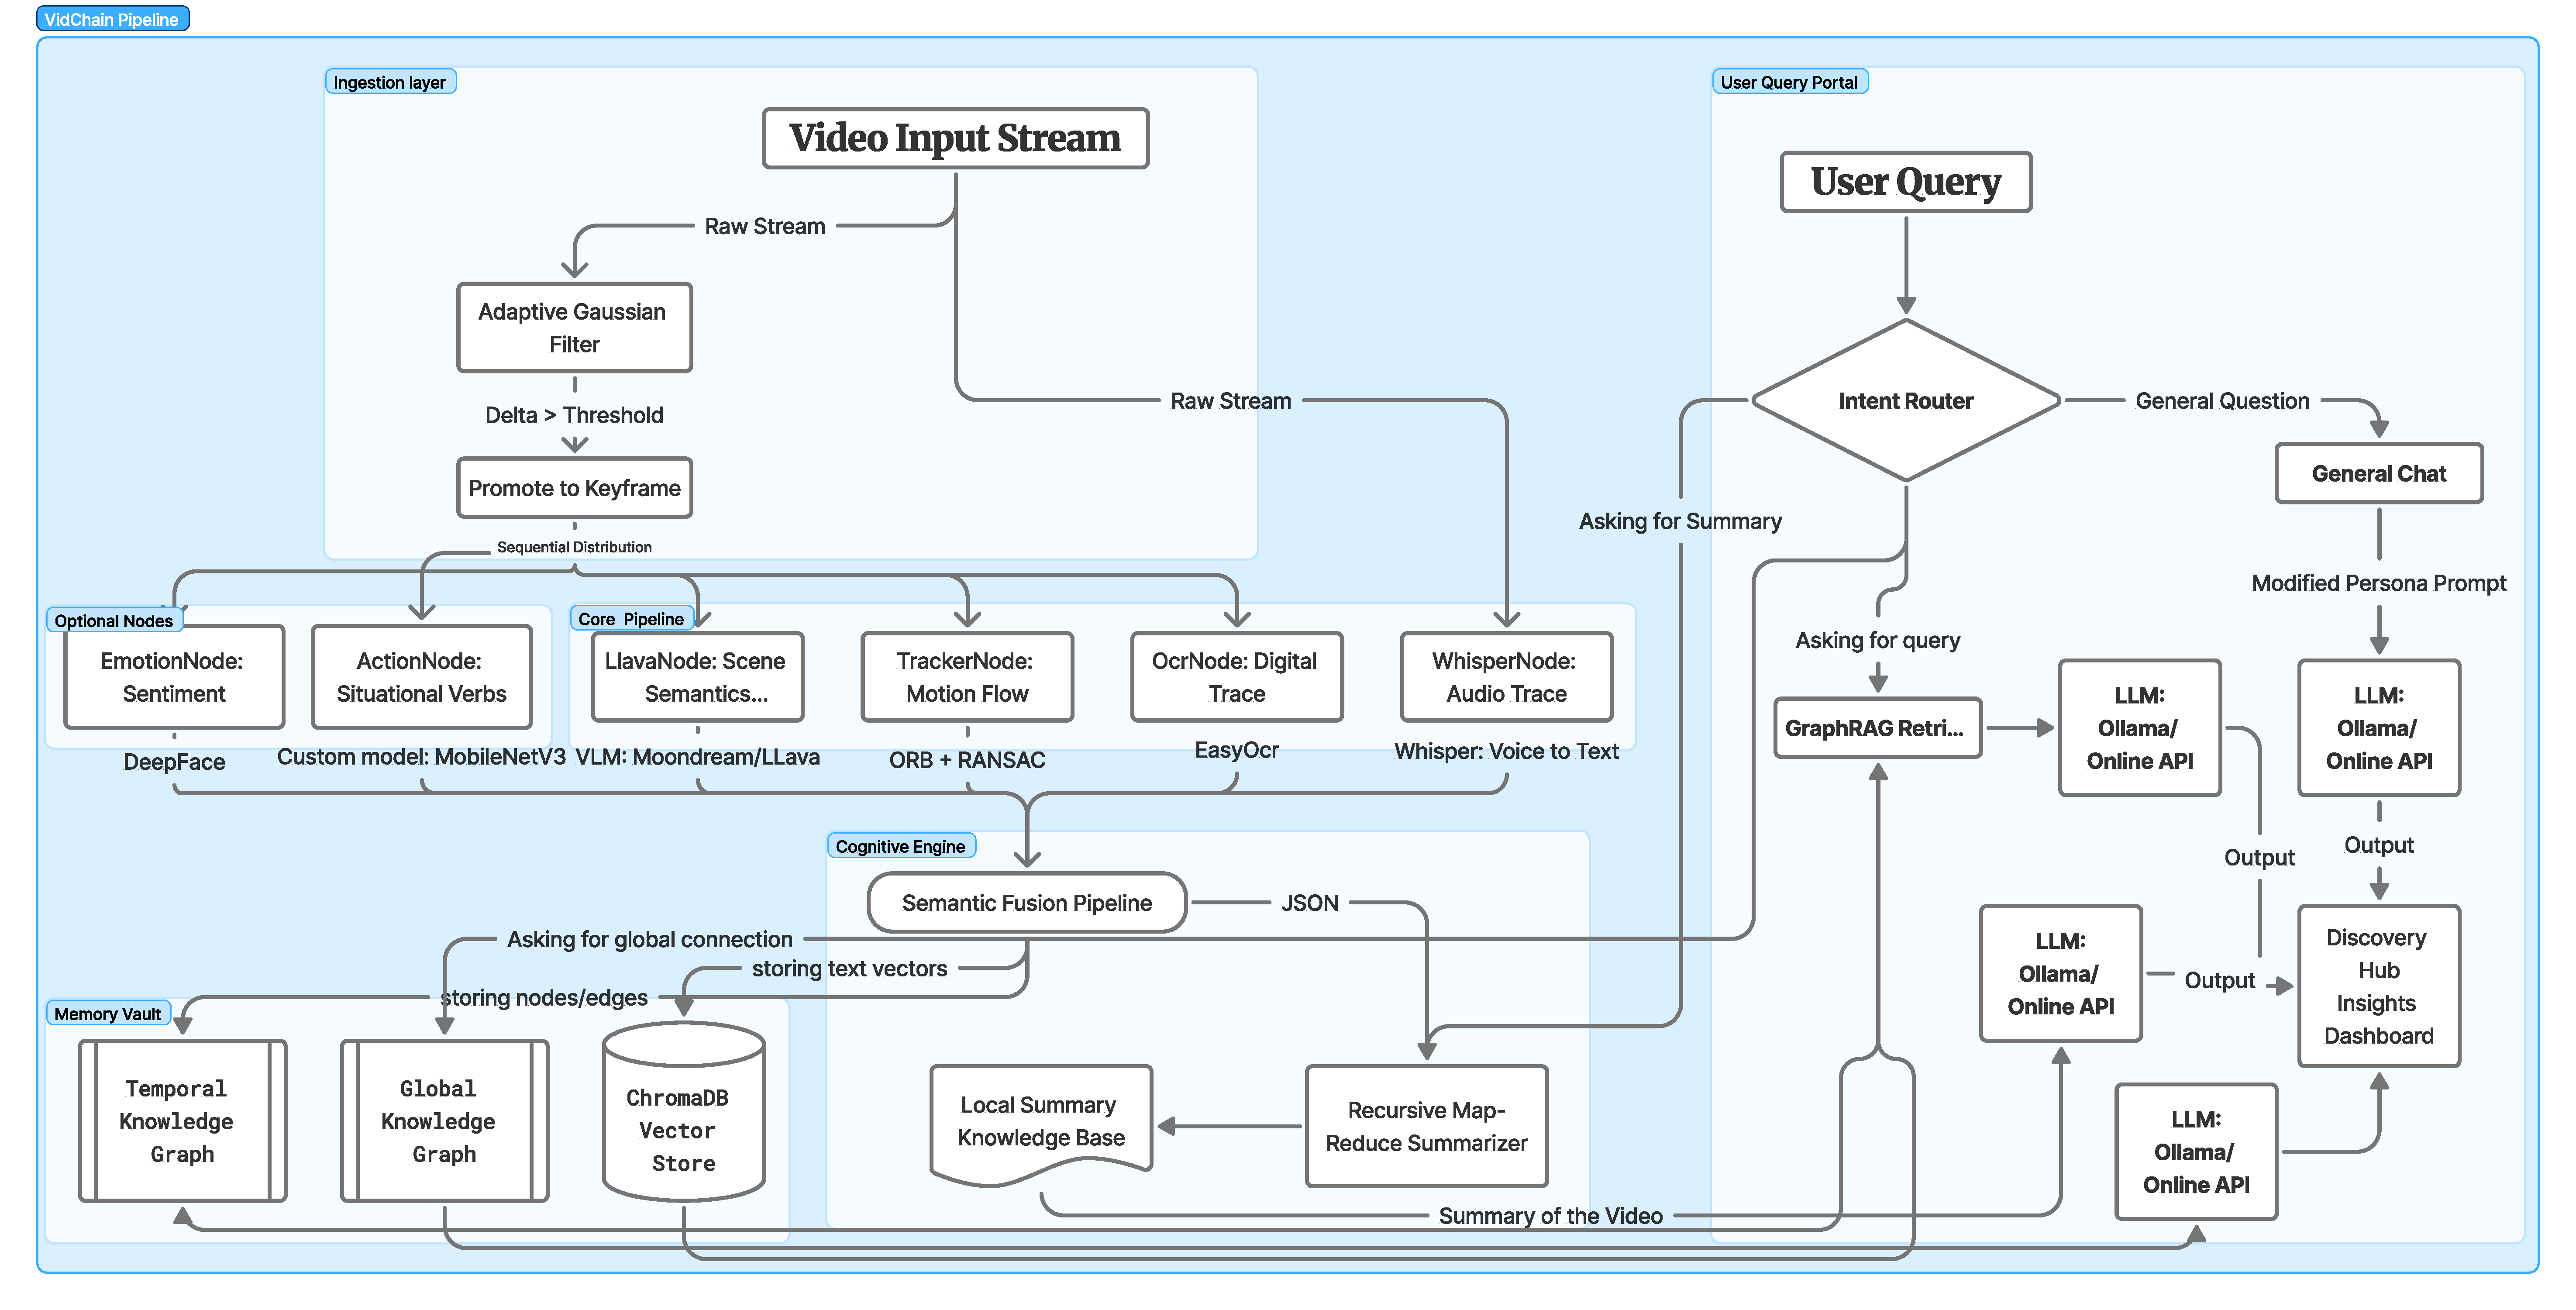
\includegraphics[width=0.95\textheight]{pipeline.pdf}
\caption{VidChain Ingestion Pipeline Process Flow}
\label{fig:ingest_flow}
\end{sidewaysfigure}
\restoregeometry

\section{Sequence Diagram: Query Lifecycle}

\begin{figure}[H]
\centering
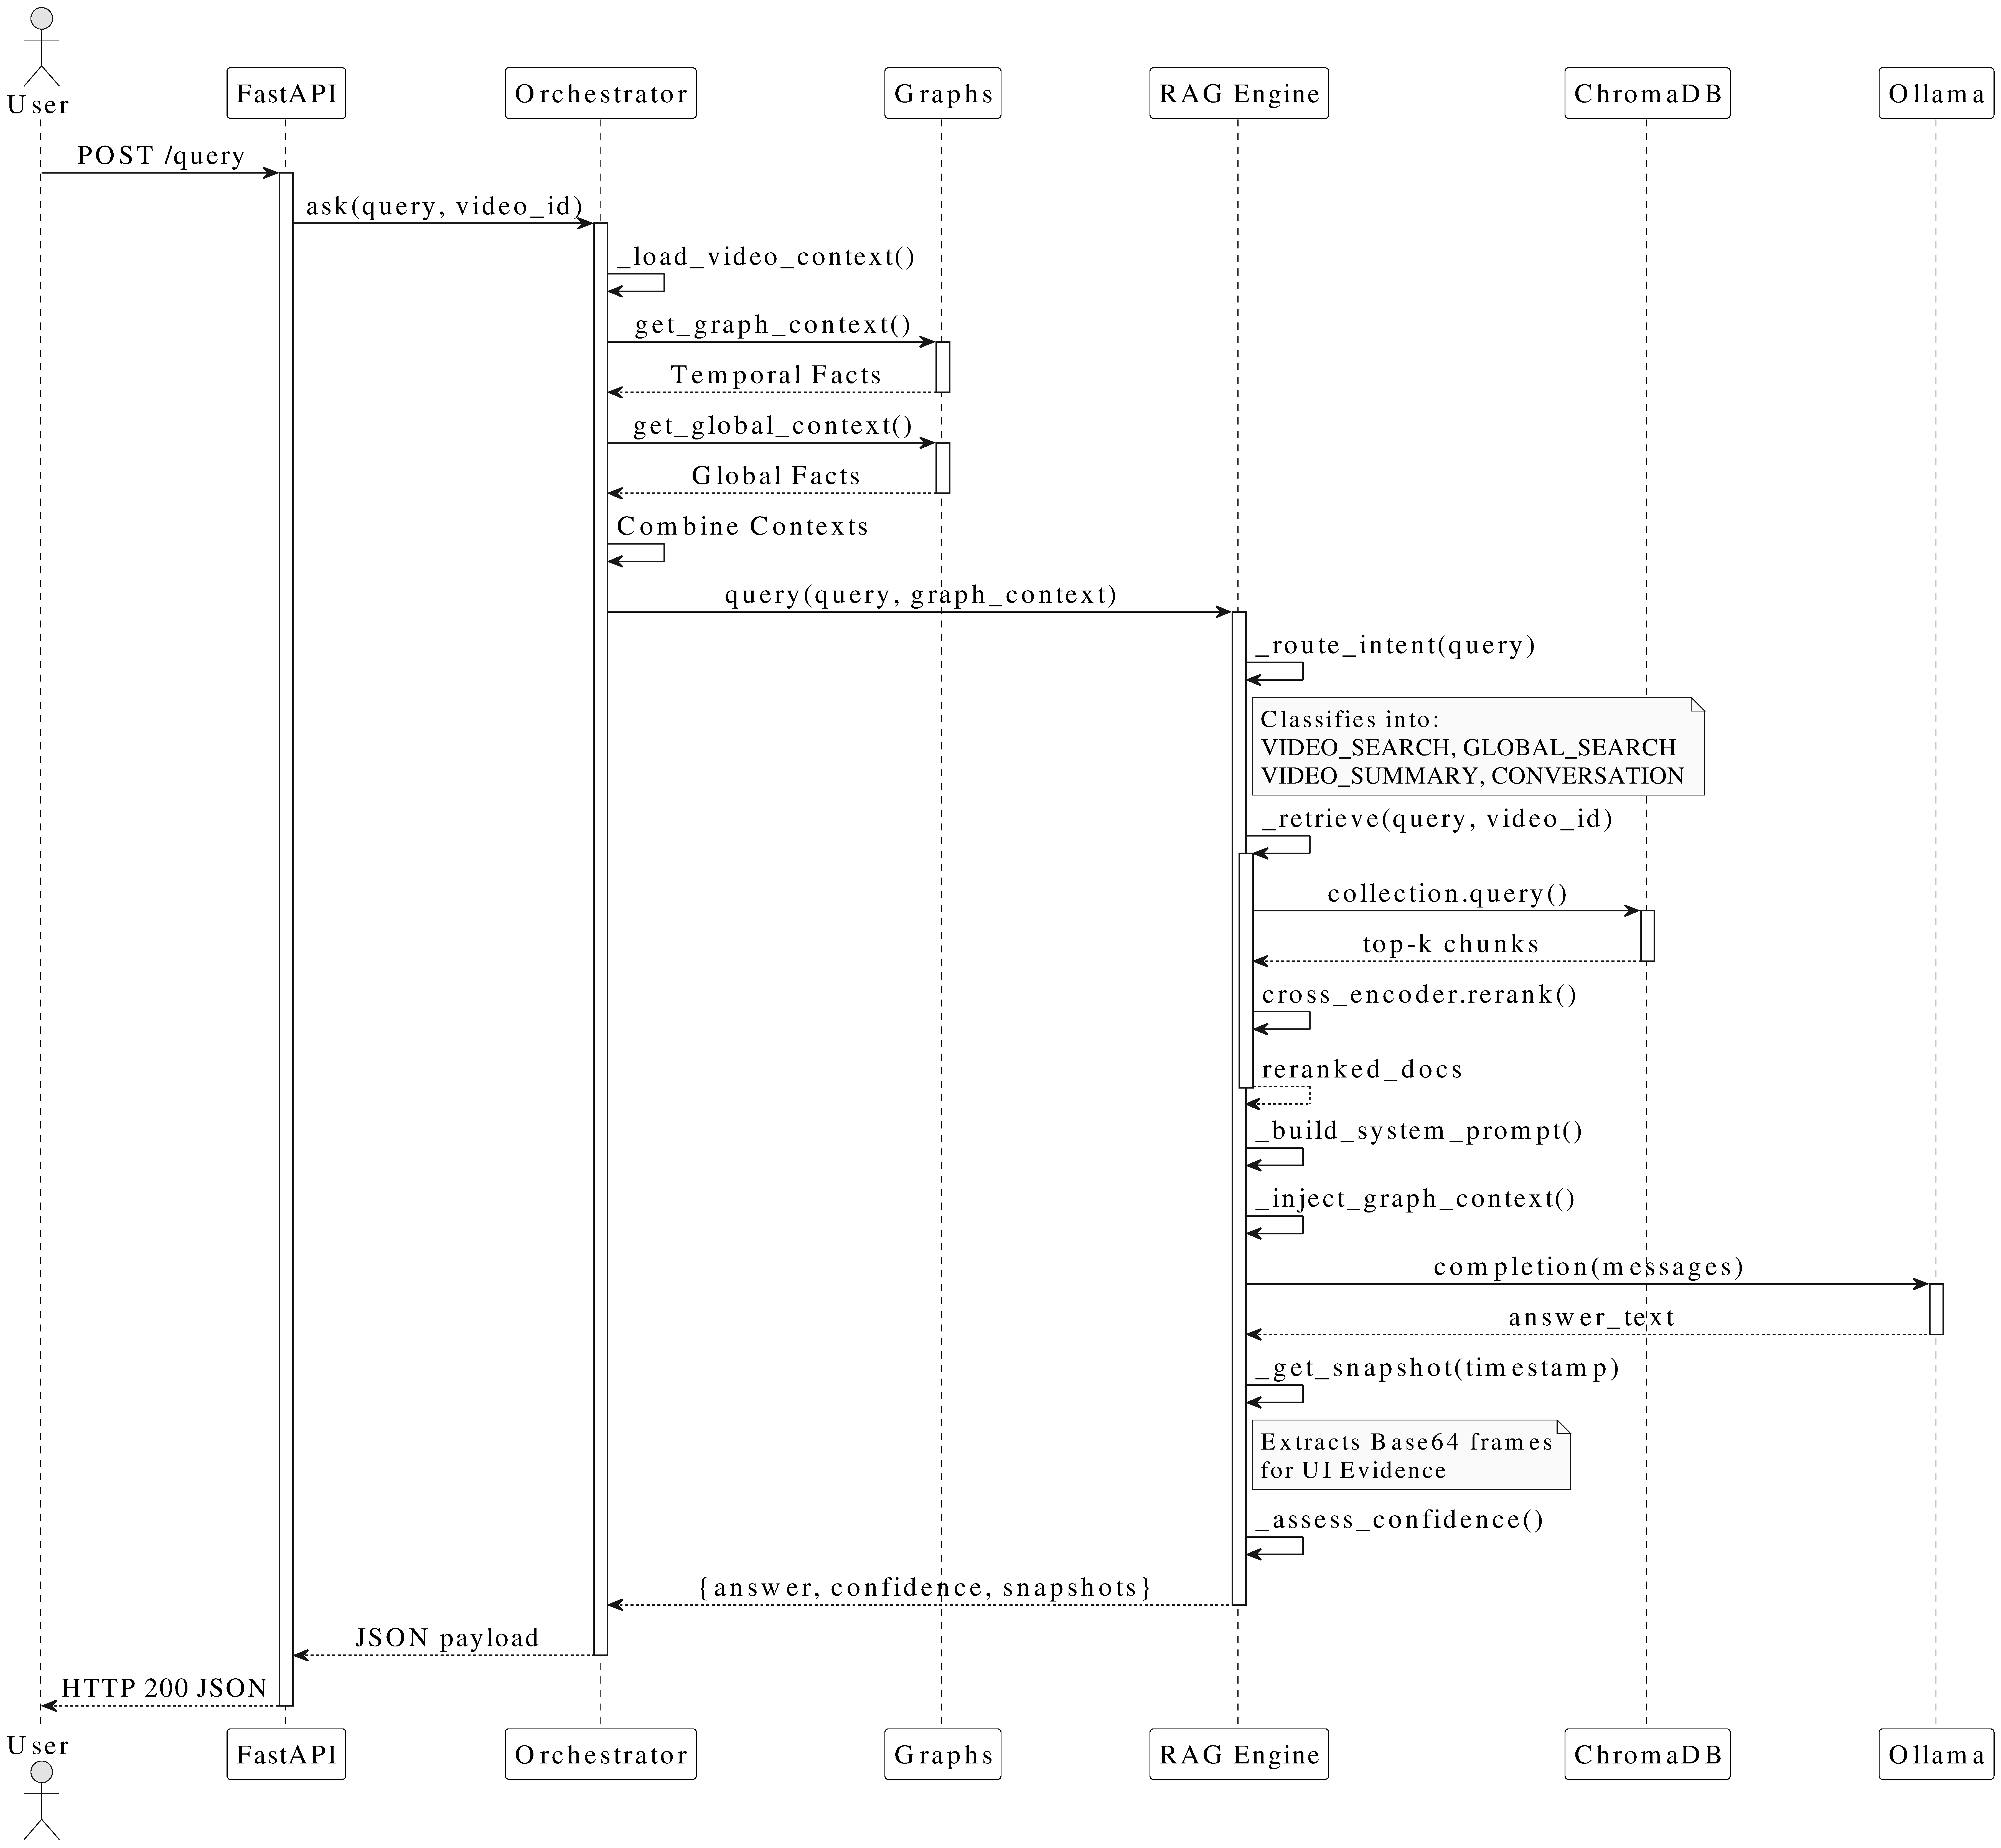
\includegraphics[angle=90, width=0.60\textheight, keepaspectratio]{sequence.pdf}
\caption{Sequence Diagram --- Full Query Lifecycle from User Request to IRIS Response}
\label{fig:sequence}
\end{figure}

\subsection{Design Justification}

The sequence diagram makes three non-obvious design decisions visible.

\textbf{Intent Routing before Retrieval.} Before any vector search is performed, the \texttt{RAGEngine} calls \texttt{\_route\_intent()} to classify the query into one of four intents: \texttt{VIDEO\_SEARCH}, \texttt{VIDEO\_SUMMARY}, \texttt{CONVERSATION}, or \texttt{GLOBAL\_SEARCH}. This matters because a summary request should not trigger ChromaDB retrieval at all and should instead route directly to the Map-Reduce Summariser. Performing retrieval first would produce a response grounded in only the top-k retrieved fragments, losing the temporal continuity that the full timeline provides.

\textbf{Graph Context Injection.} After retrieval, the system separately calls \texttt{get\_graph\_context()} on the Temporal Knowledge Graph \cite{graphrag}. The returned entity facts, including first and last seen timestamps, co-occurrence relationships, and camera motion patterns, are appended to the system prompt as a distinct block. This means the LLM receives two independent evidence sources: semantically similar fragments from ChromaDB and structured relational facts from the graph. Neither source alone is sufficient; flat vector search cannot answer ``when did person \#1 first appear?'' and a graph alone cannot answer open-ended natural language questions.

\textbf{Confidence Scoring as a Second LLM Call.} The \texttt{\_assess\_confidence()} step fires a separate, lightweight completion call asking the LLM to rate its own certainty given the retrieved context. This is the Neural Verification Pulse described in Chapter 1. Routing this as a second call rather than embedding it in the main prompt prevents the confidence reasoning from influencing the answer itself, which would introduce a self-fulfilling bias.

\section{Component Diagram}

\begin{figure}[H]
\centering
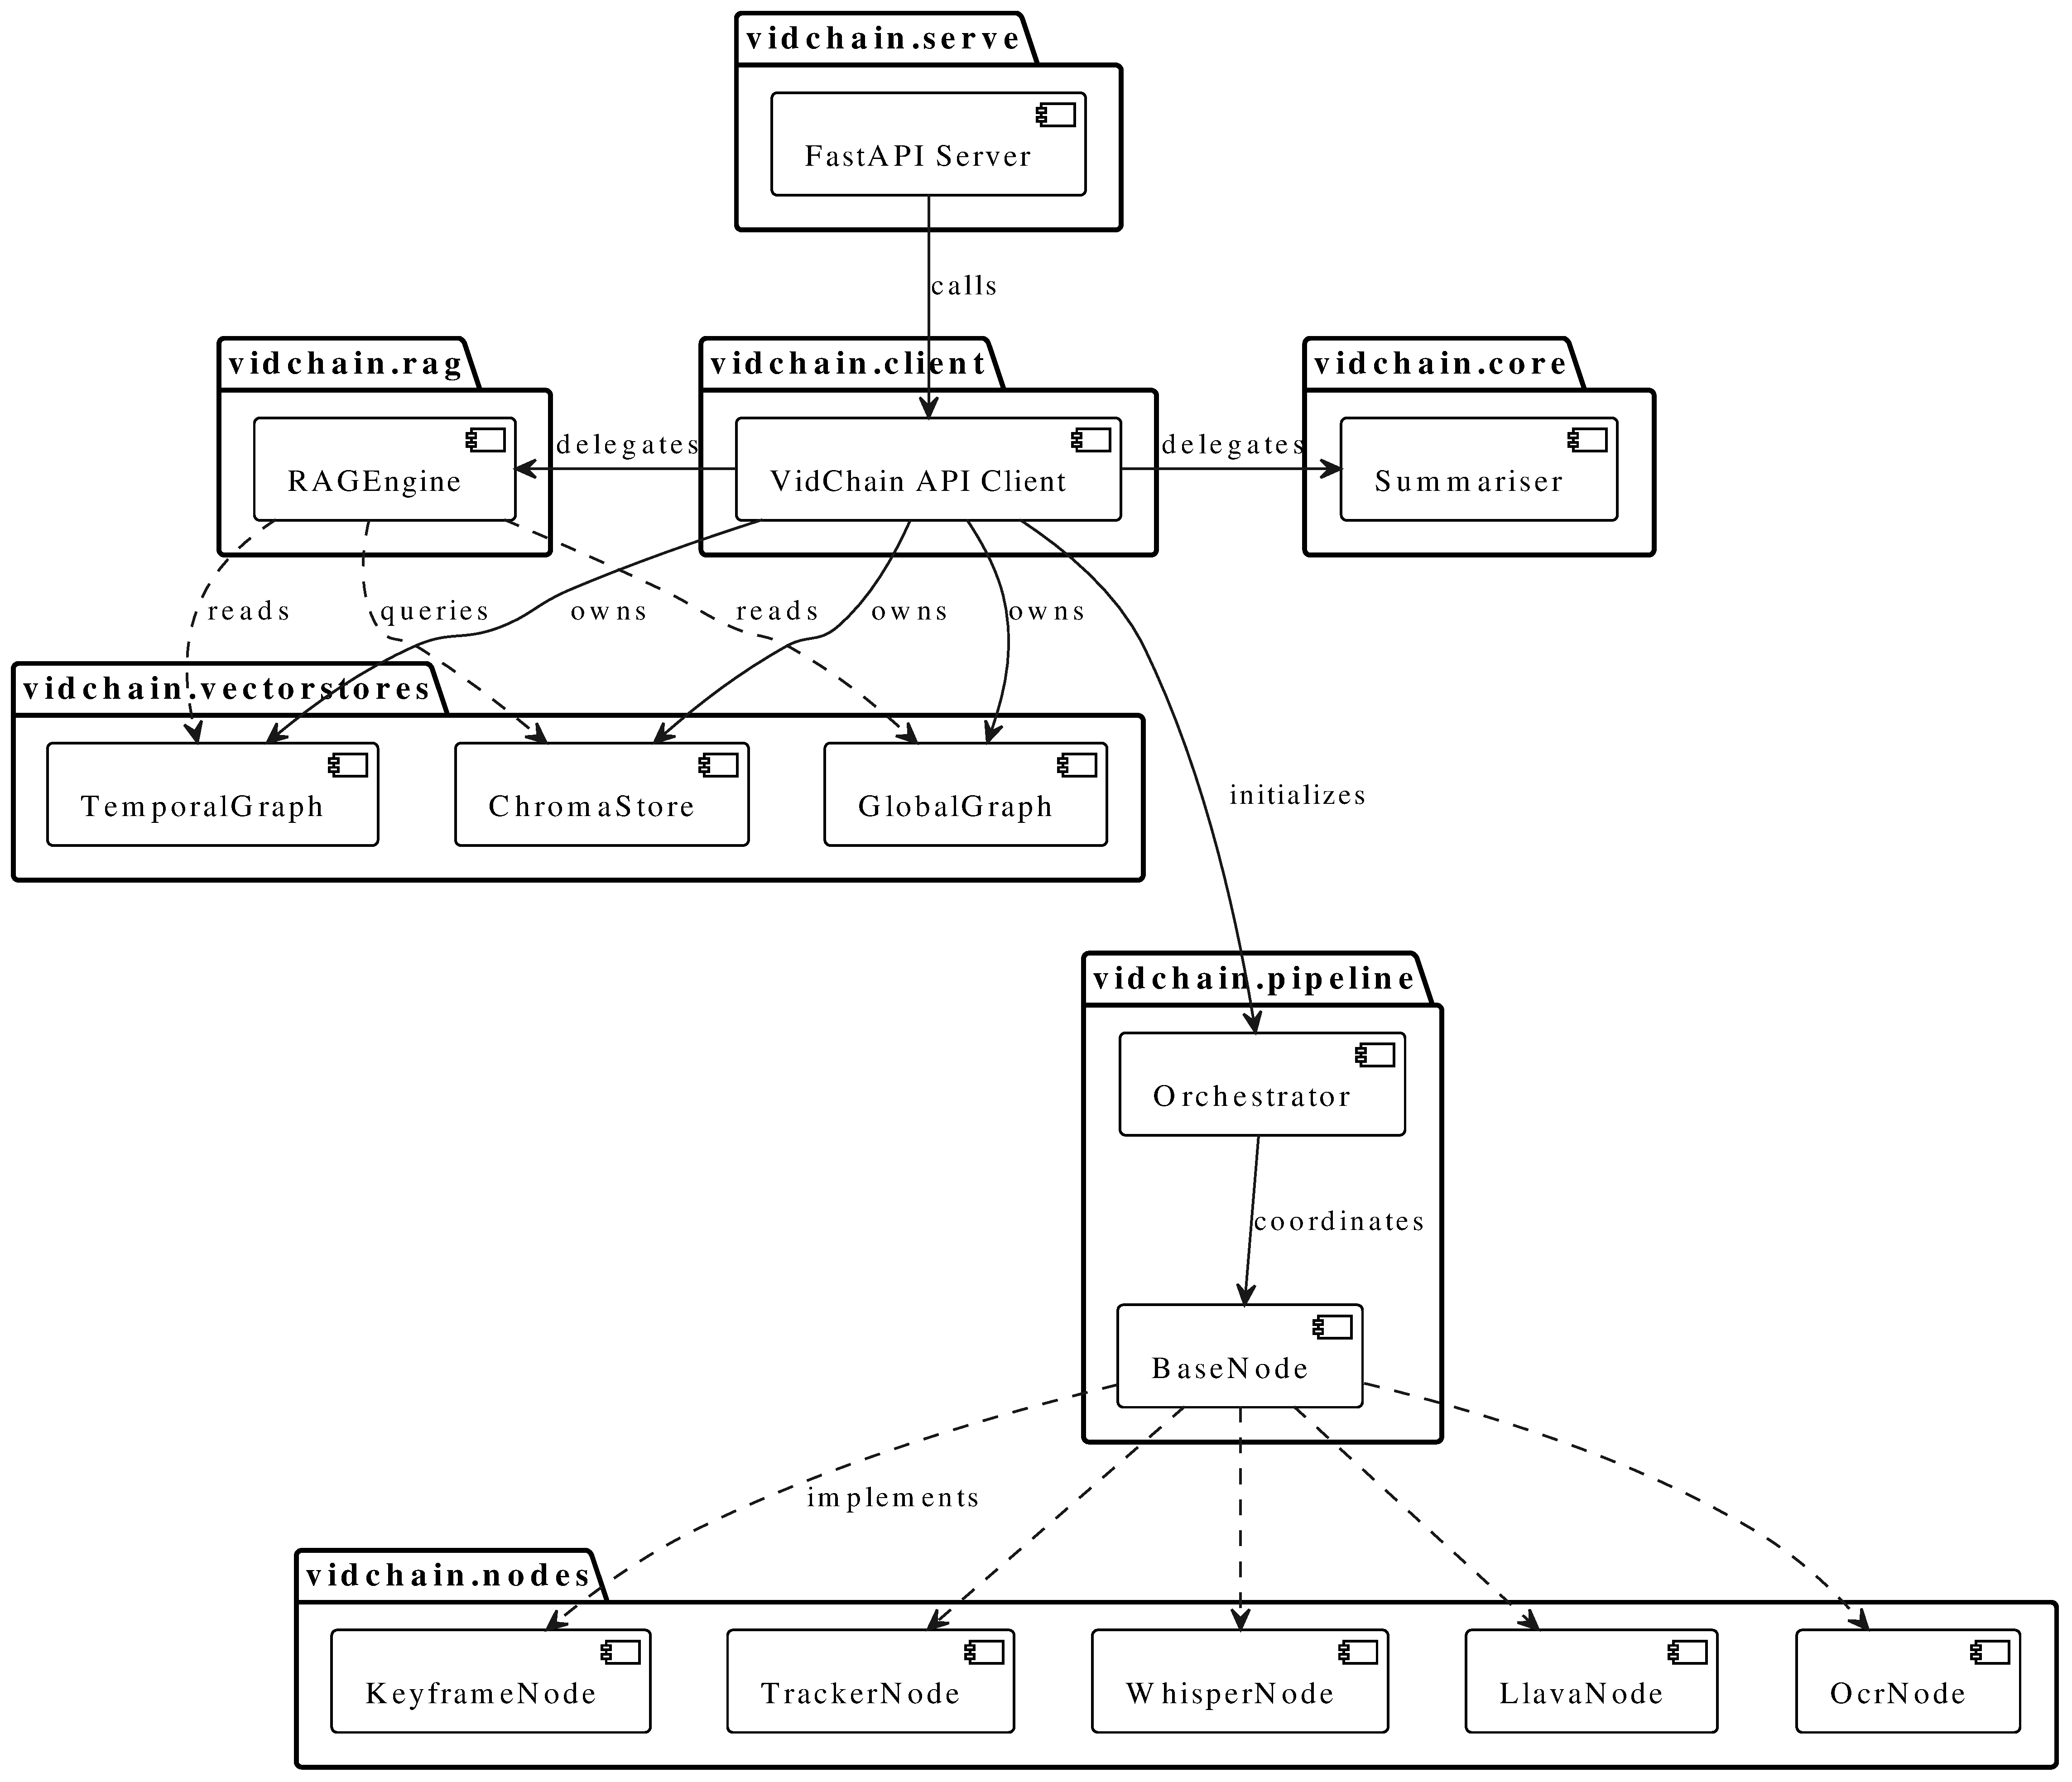
\includegraphics[angle=90, width=0.55\textheight, keepaspectratio]{component.pdf}
\caption{Component Diagram --- VidChain Package Structure and Dependencies}
\label{fig:component}
\end{figure}

The component diagram reveals two important structural properties. First, \texttt{VidChain} (in \texttt{vidchain.client}) is the single owner of all stateful components: the vector store, the knowledge graph, and the pipeline orchestrator. No other module holds references to these directly. This guarantees that memory isolation, a key requirement from Chapter 3, is enforced at the object level: swapping the active session means swapping the active \texttt{VidChain} context, which transitively swaps every downstream store.

Second, \texttt{FastAPI} (\texttt{vidchain.serve}) communicates with the system exclusively through \texttt{VidChain.ingest()} and \texttt{VidChain.ask()}. The HTTP layer has no direct access to ChromaDB, the knowledge graph, or any node. This separation means the entire intelligence pipeline can be used as a pure Python library without the server, as documented in the Quickstart Guide.

\section{State Machine Diagram: VidChain Session}

The State Machine Diagram (Figure~\ref{fig:state}) models the dynamic states a VidChain session can exist in, from initialisation to disposal. It highlights the transitions triggered by the orchestrator, including the fallback to an error state if a sensor node fails.

\begin{figure}[H]
\centering
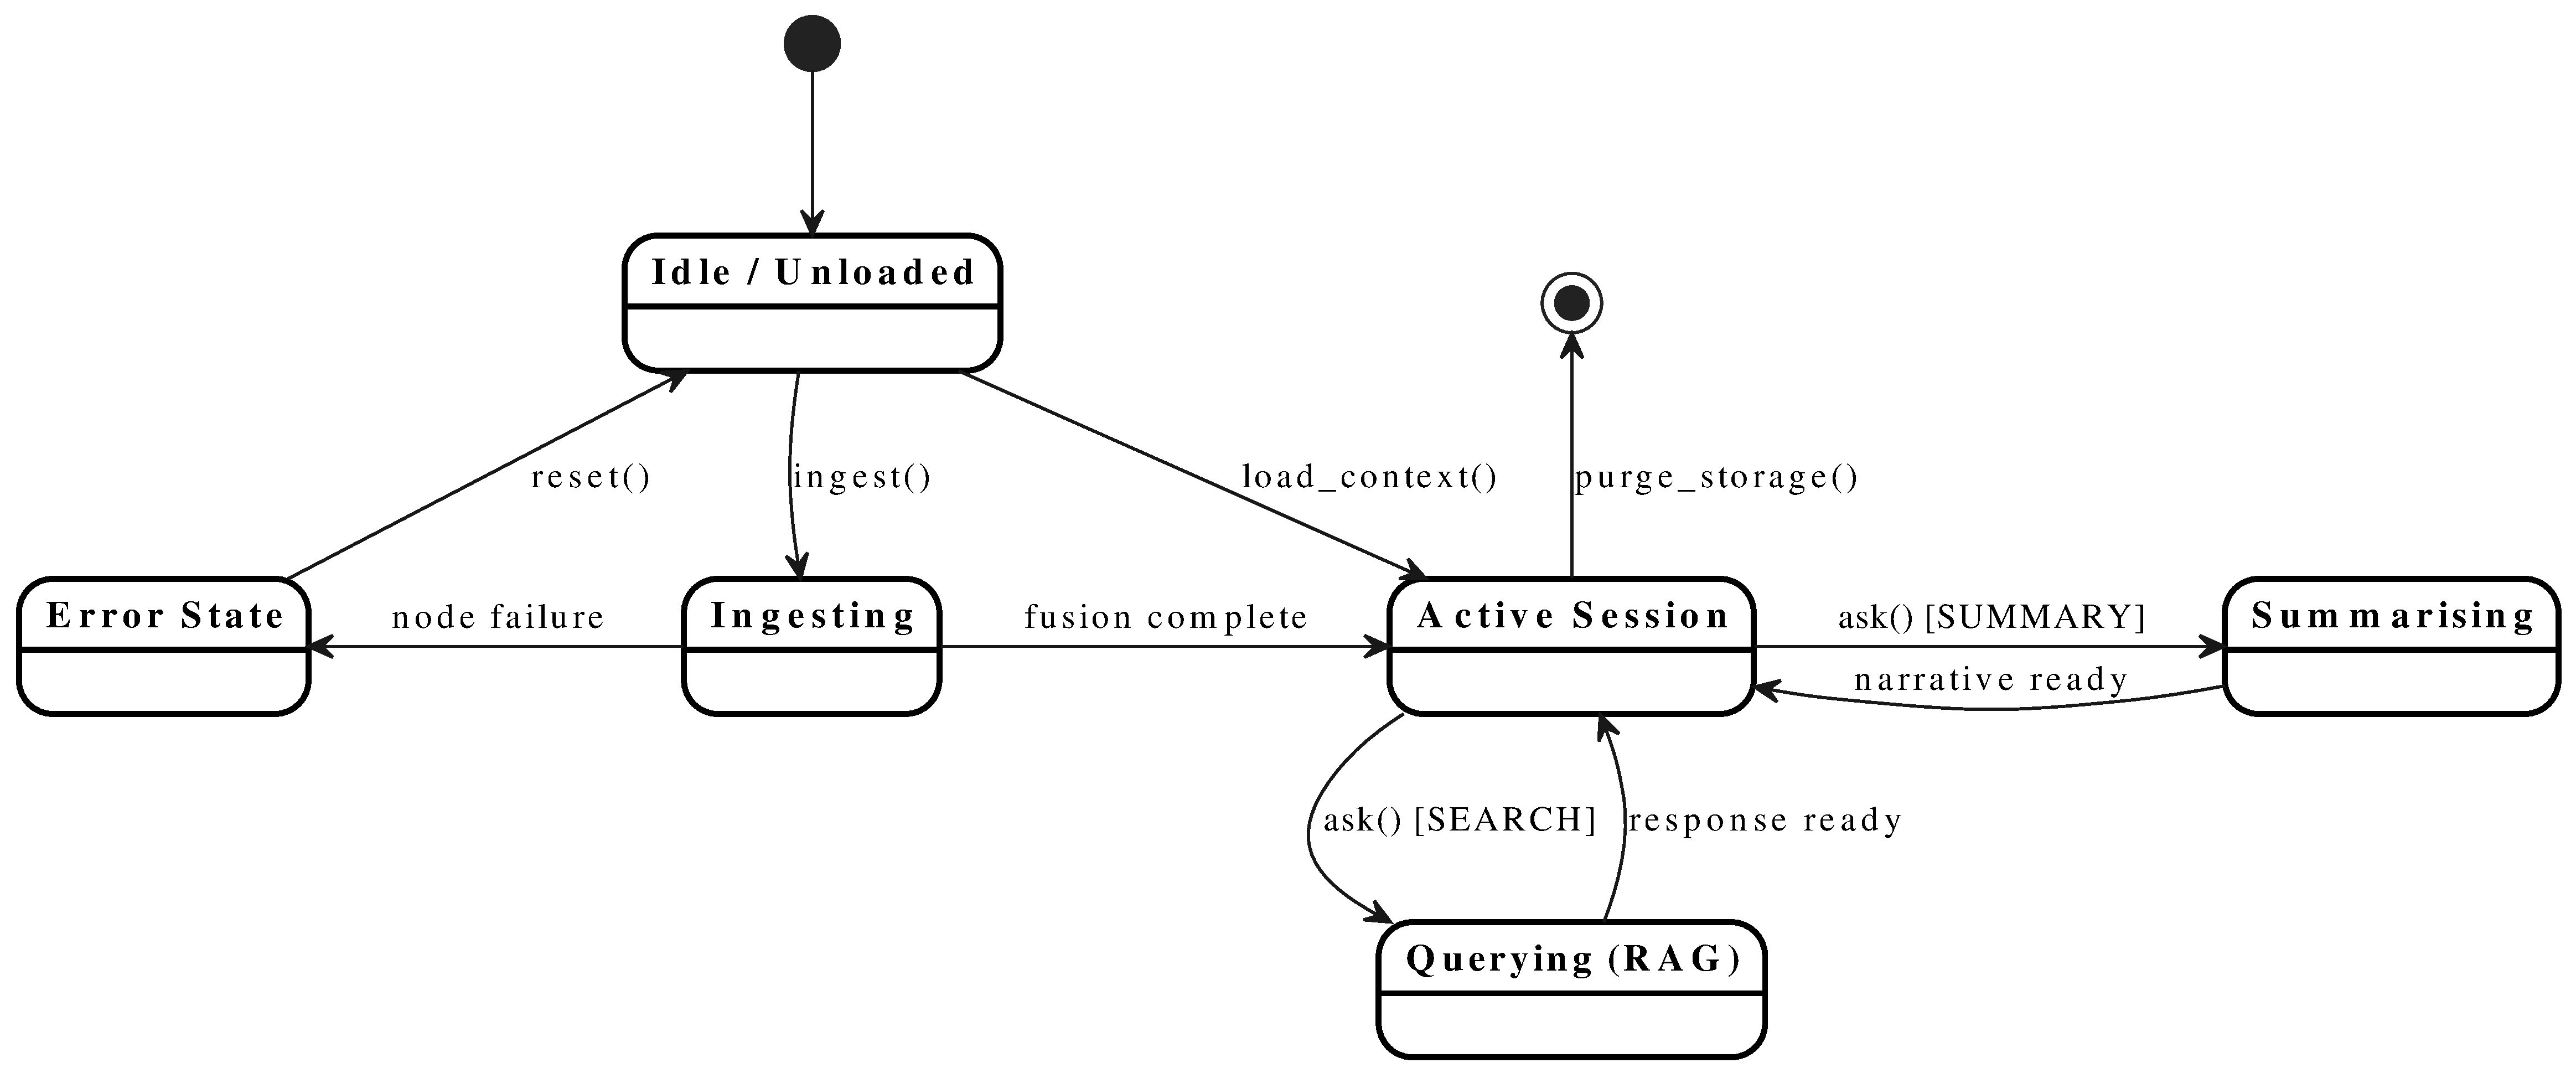
\includegraphics[width=0.55\textheight]{state.pdf}
\caption{State Machine Diagram --- VidChain Session Lifecycle}
\label{fig:state}
\end{figure}

\section{Class Diagram: Node Hierarchy}

\newgeometry{left=0.2cm, right=0.2cm, top=0.2cm, bottom=0.2cm}
\begin{sidewaysfigure}
\centering
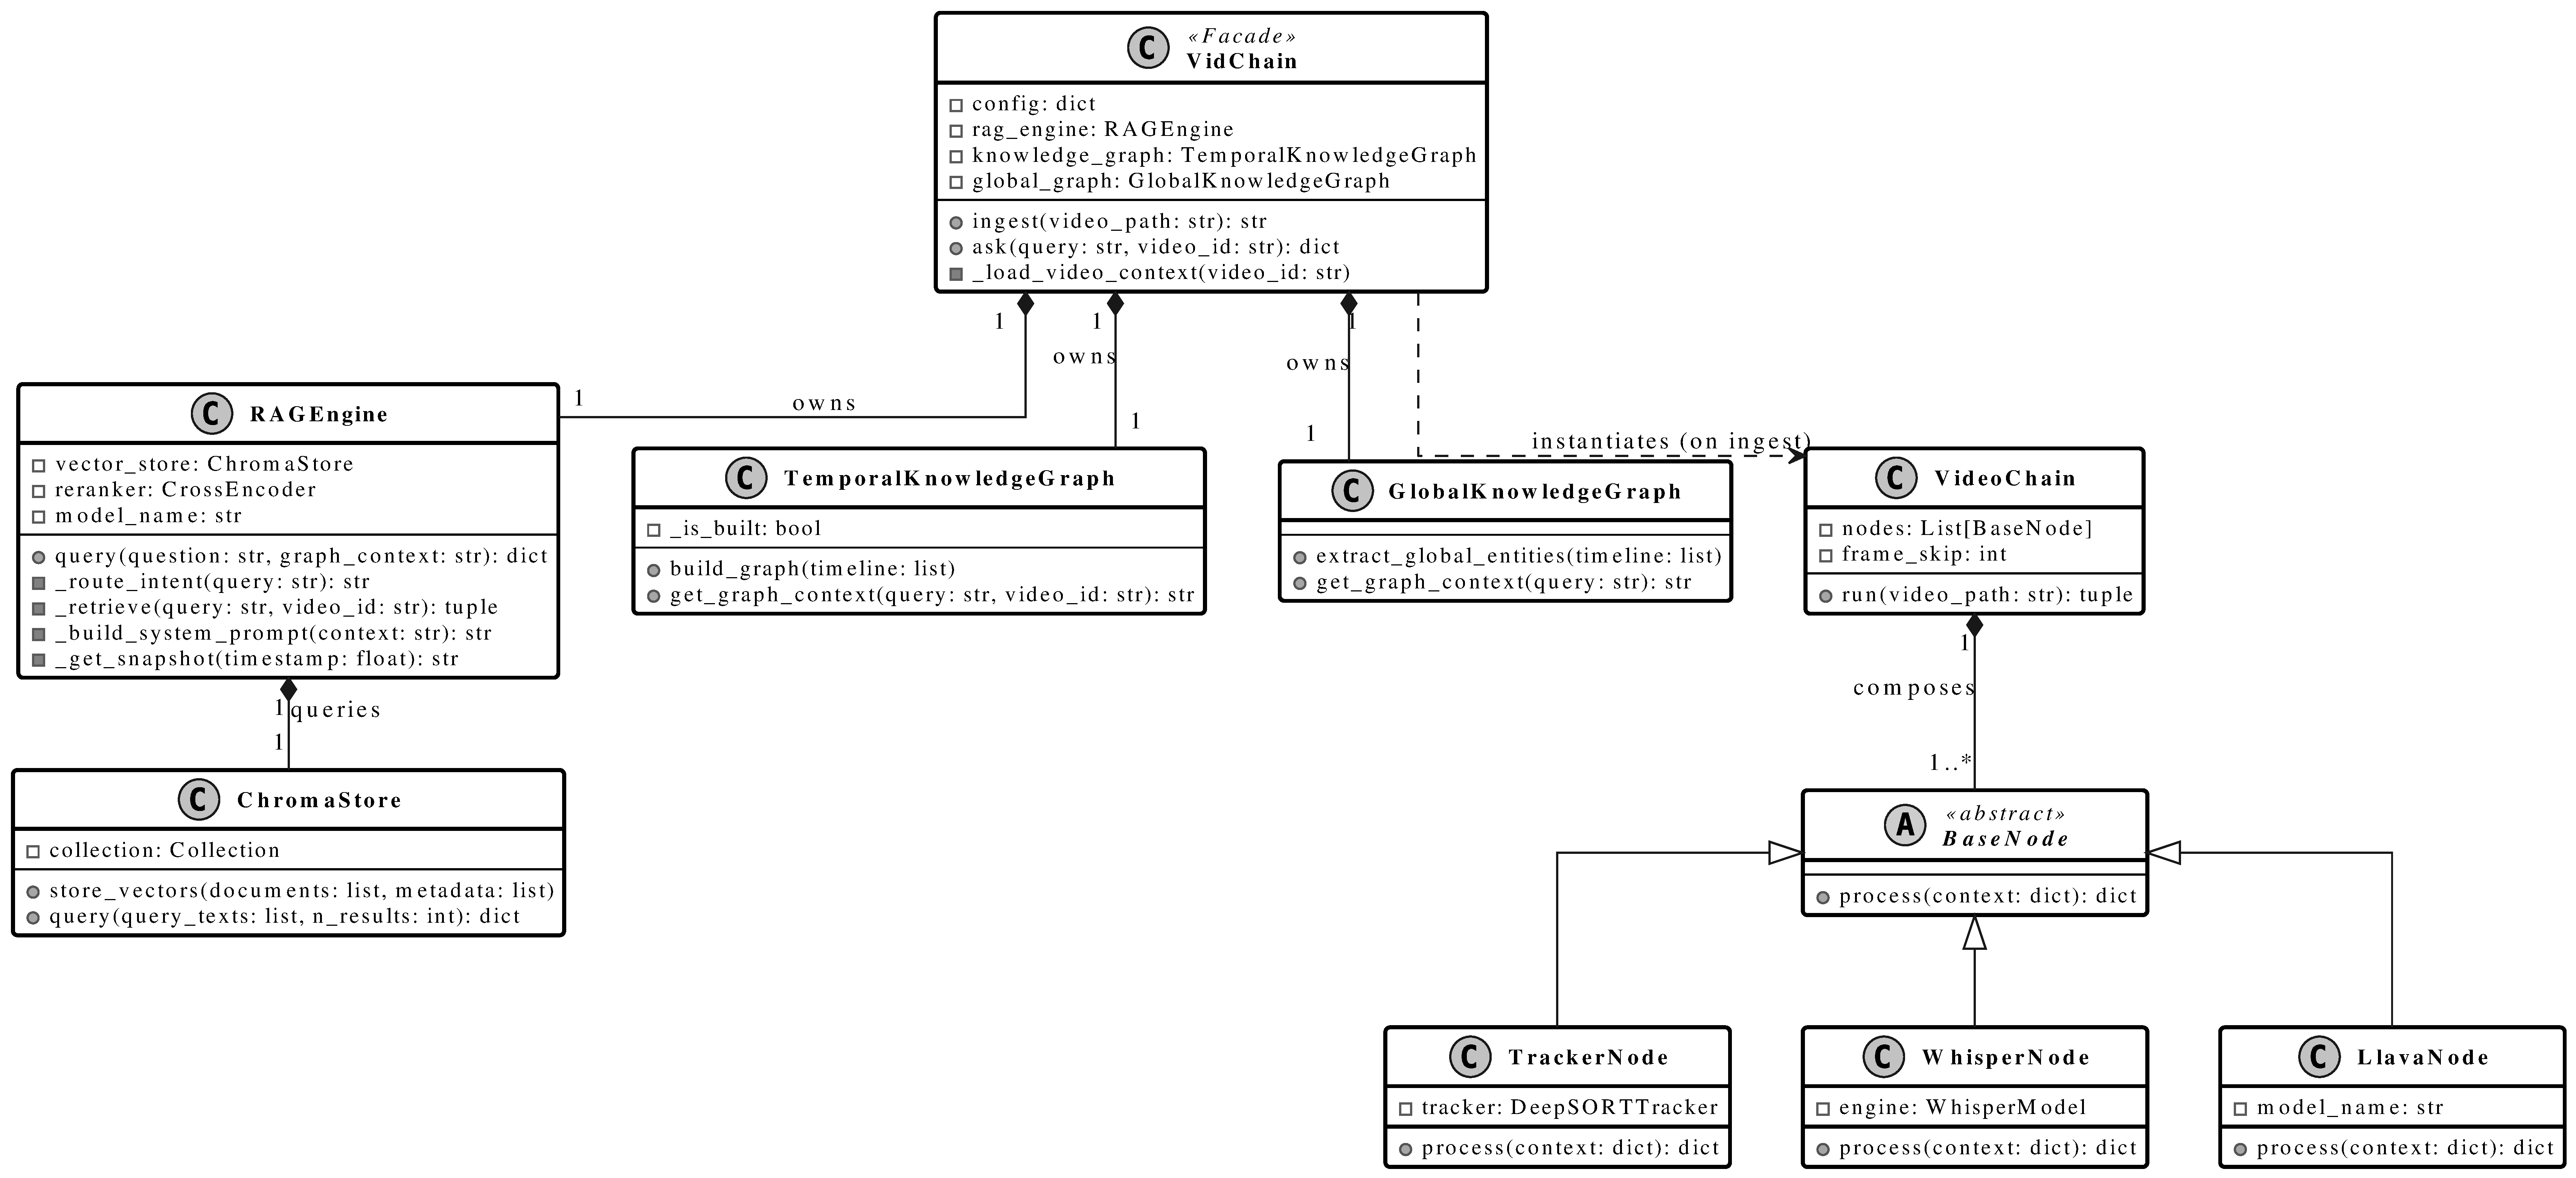
\includegraphics[width=0.90\textheight]{class.pdf}
\caption{Class Diagram --- BaseNode Hierarchy and VideoChain Composition}
\label{fig:class}
\end{sidewaysfigure}
\restoregeometry

\subsection{Design Justification: The BaseNode Contract}

The \texttt{BaseNode} abstract class defines a single method: \texttt{process(context: dict) -> dict}. This interface was chosen for its minimalism. A single-method contract imposes almost no coupling on implementors while still guaranteeing the one property the \texttt{VideoChain} orchestrator requires: that every node reads from and writes to the same shared context dictionary.

This design draws from the Chain of Responsibility pattern. Each node is responsible for one thing, knows nothing about its neighbours, and simply enriches the context it receives before passing it on. The \texttt{AdaptiveKeyframeNode} exploits this by injecting a \texttt{skip\_frame: True} flag into the context when a frame is visually redundant. Every subsequent node checks this flag and returns immediately, achieving GPU-level compute savings without any node needing to know about the keyframe logic.

The \texttt{WhisperNode} \cite{whisper} uses a \texttt{segments\_cache} to illustrate another design property: nodes can be stateful across frames. Whisper transcribes the entire audio track once on the first call and caches the result. All subsequent calls perform a cheap binary search over the cached segments to find the speech active at the current timestamp, avoiding re-running a heavy model on every frame while still providing accurate temporal alignment.

\section{The IRIS Orchestrator}

IRIS (Intelligent Retrieval \& Insight System) is not a single module but an emergent behaviour produced by the interaction of four components: the \texttt{VidChain} client, the \texttt{RAGEngine}, the \texttt{TemporalKnowledgeGraph}, the \texttt{GlobalKnowledgeGraph}, and the \texttt{VideoSummariser}. The \texttt{VidChain} client acts as the conductor: it owns the state, loads the correct per-video graph on context switch, and routes calls to the appropriate subsystem. The intelligence itself arises from the combination of vector retrieval, graph-grounded facts, and LLM synthesis \cite{ollama}.

\subsection{Memory Isolation Protocol}

A critical architectural guarantee introduced in v1.0.0 is per-session memory isolation. Each ingested video produces three isolated artefacts on disk: a ChromaDB \cite{chromadb} collection entry keyed by \texttt{video\_id}, a pickled NetworkX \cite{networkx} graph at \texttt{knowledge\_graphs/graph\_\{video\_id\}.pkl}, and a JSON knowledge base at \texttt{knowledge\_bases/\{video\_id\}.json}. When the user switches sessions, \texttt{VidChain.\_load\_video\_context()} hot-swaps the active graph by deserialising the correct \texttt{.pkl} file. ChromaDB queries are always filtered with a \texttt{where: \{video\_id: ...\}} clause. This guarantees that no information from one video session can bleed into the retrieval results of another, a property referred to in the codebase as Cross-Video Noise prevention.

\subsection{Recursive Map-Reduce Summarisation}

The \texttt{VideoSummariser} solves the Context Window Wall through a three-phase process inspired by the MapReduce programming model \cite{mapreduce}. In the Map phase, the full timeline is split into word-budget chunks (default: 1,500 words per chunk) and each chunk is independently summarised by the LLM into a dense chapter summary. In the Reduce phase, chapter summaries are grouped into batches of five and recursively collapsed until only one summary remains. In the Polish phase, the final collapsed summary is passed through a formatting prompt that applies the IRIS narrative voice: professional, chronological, and evidence-grounded. The recursion depth scales logarithmically with video length, meaning a three-hour lecture requires at most three or four LLM calls to produce the final report, regardless of the original token count.

\section{GraphRAG: Temporal Knowledge Graph}

The \texttt{TemporalKnowledgeGraph} is built on NetworkX \cite{networkx} and populated immediately after every \texttt{ingest()} call. The graph contains three node types: timestamp nodes (one per timeline entry), entity nodes (persons, objects, and OCR text strings), and camera behaviour nodes (panning, tilting, zooming). Edges encode relationships: \texttt{detects} (timestamp $\to$ entity), \texttt{co-occurs} (entity $\leftrightarrow$ entity), \texttt{screen\_shows} (timestamp $\to$ OCR text), and \texttt{camera\_behavior\_is} (timestamp $\to$ motion type).

This structure enables queries that are impossible for flat vector search \cite{colbert}. A question such as ``did the same person appear in both the opening and closing segments?'' requires knowing the first-seen and last-seen timestamps of a tracked entity, information stored as node attributes in the graph but which would otherwise require scanning the entire ChromaDB collection. The \texttt{get\_graph\_context()} method serialises the most relevant graph facts into a natural language block injected directly into the LLM's system prompt, grounding the response in verified structural evidence rather than probabilistic retrieval alone \cite{graphrag}.

\section{ER Diagram: Knowledge Graph Schema}

The Entity-Relationship (ER) diagram (Figure~\ref{fig:er}) defines the structural schema of the VidChain reasoning layer. It illustrates how the three databases (ChromaDB, Local Graph, and Global Graph) are architecturally linked through a shared \texttt{video\_id} and temporal index.

\begin{figure}[H]
\centering
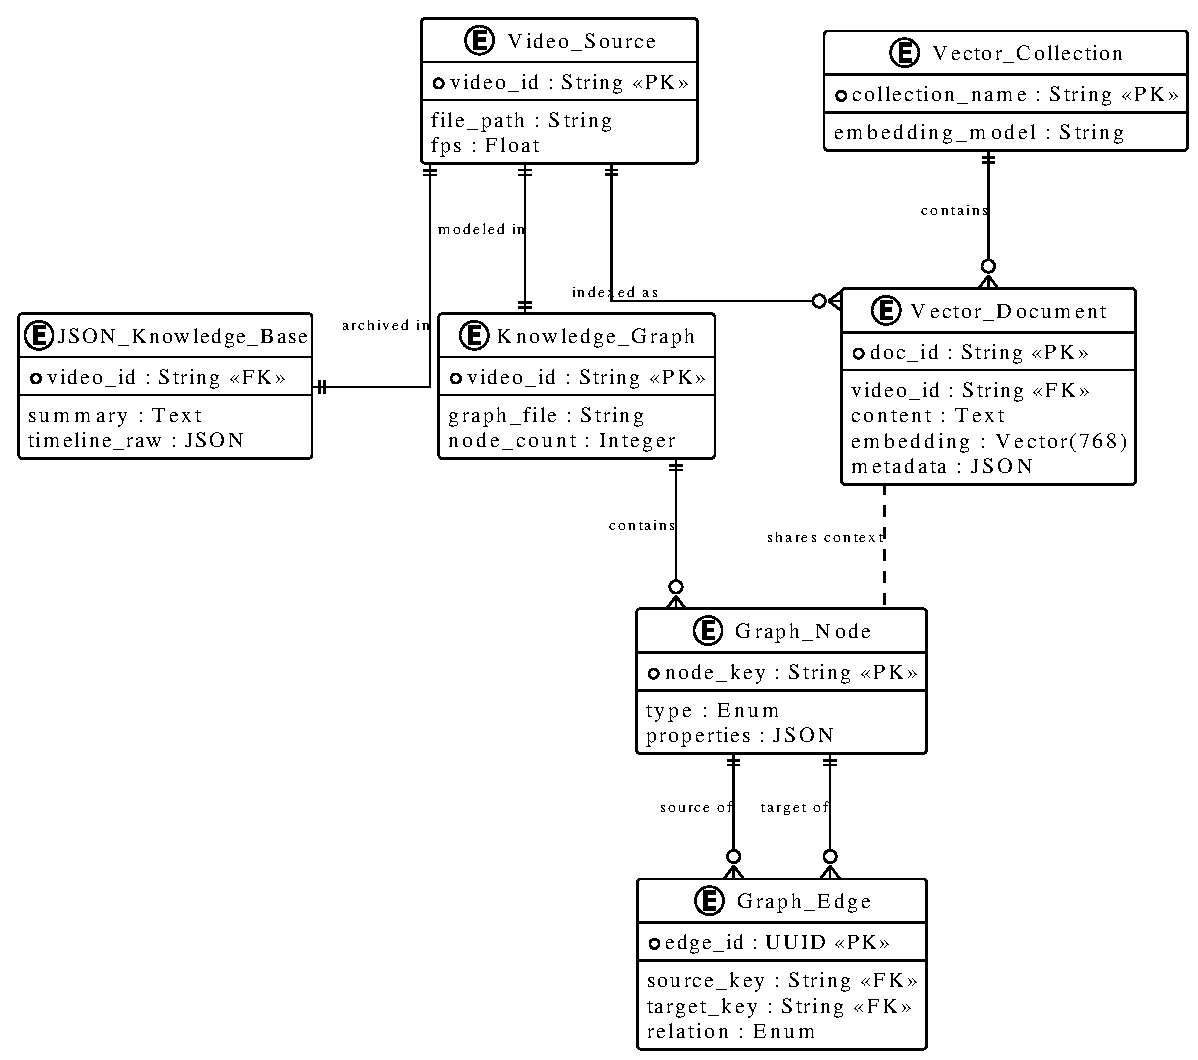
\includegraphics[width=0.85\textwidth]{ER.pdf}
\caption{ER Diagram --- Relational Schema of the Temporal Knowledge Graph}
\label{fig:er}
\end{figure}

The schema highlights the many-to-many relationship between timestamp nodes and entity nodes, which is the basis for GraphRAG's ability to track object persistence. By storing \texttt{first\_seen} and \texttt{last\_seen} attributes on the entity nodes, the system can perform $O(1)$ lookups for temporal duration queries, which would otherwise require $O(N)$ scans in a traditional vector database.


\section{Summary}

This chapter has presented the full architectural design of VidChain across four levels of abstraction. The Late-Fusion paradigm was justified as the only viable approach for edge hardware, and its consequences, including independent nodes, shared context dictionaries, and modality-specific failure isolation, were traced through the component and class diagrams. The sequence diagram exposed three deliberate design decisions: intent routing before retrieval, dual-source evidence injection combining vector and graph retrieval, and confidence scoring as a second-pass verification step. The IRIS orchestrator's two most significant subsystems, the Memory Isolation Protocol and the Recursive Map-Reduce Summariser, were described with sufficient detail to motivate the implementation choices documented in Chapter 5.